\documentclass[a4paper,twoside,12pt,hidelinks]{article}
\usepackage{float}
\usepackage[numbered, framed]{mcode}
\usepackage[titletoc]{appendix}
\usepackage[skip=5pt]{subcaption}
\lstset{aboveskip=0pt,belowskip=8pt}
\usepackage[a4paper,left=2cm,right=2cm,top=2cm,bottom=2cm]{geometry}
\usepackage[parfill]{parskip}
\usepackage{graphicx}
\usepackage[export]{adjustbox}
\usepackage{amsmath,amssymb}
\usepackage{commath}
\usepackage{multirow}
\usepackage{setspace}
\usepackage{tabularx}
\usepackage{bm}
\setlength{\belowcaptionskip}{-5pt}
\newcolumntype{Y}{>{\centering\arraybackslash}X}
\usepackage{pdflscape}
\usepackage[nodayofweek,level]{datetime}
\usepackage{wrapfig}
\graphicspath{{figures/}}
\usepackage{titlesec}
\setcounter{secnumdepth}{4}
\titleformat{\paragraph}
{\normalfont\normalsize\bfseries}{\theparagraph}{1em}{}
\titlespacing*{\paragraph}
{0pt}{3.25ex plus 1ex minus .2ex}{1.5ex plus .2ex}
\usepackage[nottoc]{tocbibind}
\usepackage[colorlinks=false]{hyperref}

\title{Audio Signal Zoom for Small Microphone Arrays}
\author{Chi Hang Leung}

\begin{document}
\begin{titlepage}

\newcommand{\HRule}{\rule{\linewidth}{0.5mm}} % Defines a new command for the horizontal lines, change thickness here

%----------------------------------------------------------------------------------------
%	LOGO SECTION
%----------------------------------------------------------------------------------------

\includegraphics[width=8cm]{imperial.png}\\[1cm] % Include a department/university logo - this will require the graphicx package
 
%----------------------------------------------------------------------------------------

\center % Center everything on the page

%----------------------------------------------------------------------------------------
%	HEADING SECTIONS
%----------------------------------------------------------------------------------------

\textsc{\LARGE MEng Final Year Individual Project \\[0.5cm] Interim Report}\\[1.5cm] % Name of your university/college
\textsc{\Large Imperial College London}\\[0.5cm] % Major heading such as course name
\textsc{\large Department of Electrical and Electronic Engineering}\\[0.5cm] % Minor heading such as course title

%----------------------------------------------------------------------------------------
%	TITLE SECTION
%----------------------------------------------------------------------------------------
\makeatletter
\HRule \\[0.4cm]
{\Large \bfseries \@title}\\[0.4cm] % Title of your document
\HRule \\[1.5cm]
 
%----------------------------------------------------------------------------------------
%	AUTHOR SECTION
%----------------------------------------------------------------------------------------

\begin{minipage}{0.4\textwidth}
\begin{flushleft} \large
\emph{Author:}\\
\@author \\[1.2em]
\emph{CID:} \\
00978321
\end{flushleft}
\end{minipage}
~
\begin{minipage}{0.4\textwidth}
\begin{flushright} \large
\emph{Supervisor:} \\
Dr. Patrick Naylor \\[1.2em] % Supervisor's Name
\emph{Second Marker:} \\
Mr. Mike Brookes % second marker's name
\end{flushright}
\end{minipage}\\[2cm]
\makeatother

% If you don't want a supervisor, uncomment the two lines below and remove the section above
%\Large \emph{Author:}\\
%John \textsc{Smith}\\[3cm] % Your name

%----------------------------------------------------------------------------------------
%	DATE SECTION
%----------------------------------------------------------------------------------------

{\large \today}\\[2cm] % Date, change the \today to a set date if you want to be precise

\vfill % Fill the rest of the page with whitespace

\end{titlepage}
\pagebreak
\clearpage
\setcounter{page}{1}
\onehalfspacing
\setcounter{tocdepth}{2}
\tableofcontents
\spacing{1.1}
\newpage
\section{Introduction}
This project seeks to investigate algorithms to achieve acoustic zooming in the context of smartphones. The purpose of the project is to capture audio samples containing multiple speakers, which then could be used to develop an algorithm that can zoom (in audio terms) towards one selected sound source. The nature of the project is software-based, with MATLAB being the main platform for development.

This report begins with the background and the initiatives of the project, followed by the background research on the existing techniques. The report then provides a detailed layout of the project plan with deliverables, as well as the progress up to date. It concludes with the vision of future works in the remainder of the project.
\section{Background}
\subsection{Scope and Aims}
Often one would take videos using their smartphones to capture the precious moments, such as parties and ceremonies. However, inevitably there would be interference, where one would zoom the camera towards the point of interest to avoid the unwanted images. A similar question aroused - whether one can make the sound of the speaker of interest closer in the context of smartphones.

This problem resonates with the `Cocktail Party Problem' illustrated by Colin Cherry in 1953 \cite{Cherry1953SomeEars}. Human brains have the ability to amplify the sound coming from a certain direction using their phase difference of arrival to two ears. Hence, under noisy environments such as cocktail party, with a lot of people speaking, the person one is chatting with is still audible. Over the years, different signal processing techniques have been developed to try replicating the processing by human ears and brains to microphones and computer. \cite{Mitchell1971SignalEffect} Despite being an established technique to achieve audio zoom, beamforming technique requires large microphone arrays typically to provide a narrow and precise beam. For small devices like phones in this project's context, developing alternative approaches is required, which is the main focus of the project. The aims of the project include the following: 
\begin{itemize}
\item Capturing audio samples containing more than one person talking
\item Developing an algorithm that can zoom (in audio terms) towards the speaker of interest, with the primary approach being using spatio-temporal processing with oracle mask
\item Evaluating the performance of the algorithm (e.g. in terms of speech quality, distortion)
\end{itemize}
It is expected that by the end of the project, a successful demonstration of the algorithm using MATLAB on sample data to perform audio zoom towards a specific sound source would be performed.

An important to note here is regarding to the first aim to capture audio examples. Instead of real-life recording using smartphones, a room acoustics simulation environment using anechoic speeches as input is preferred. This would allow a more rapid verification environment for the algorithm, as one can easily modify details such as position, directivity or loudness of the sound source and generate a new set of test data. While real-life data would be the ultimate goal of the project, at the beginning stages, the flexibility and rapidness in prototyping leads to the selection of software simulation.

Despite the ultimate aim to apply the acoustic zoom in scenarios containing multiple speakers, the scope of the project would be focusing on the cases involving two speakers, with the vision that the algorithm can be potentially extended to a multi-source environment. Besides, as the initiation of the project is to apply the acoustic zoom algorithm on mobile phones, which mostly have a dual-omnidirectional-microphone set-up \cite{Jeub2012NoiseDifferences}, the number of omnidirectional microphones is chosen to be two, one at the top and one at the bottom of the smartphone.

\begin{figure}[H]
\centering
\includegraphics[width=0.4\textwidth]{mobilephone}
\caption{Example of microphones location in a smartphone (Figure modified from \cite{Jeub2012NoiseDifferences})}
\label{fig:mobilephone}
\end{figure}

\subsection{Assumptions}
The stated problem can be decomposed into two parts, one part as identifying the direction of the speaker with respect to the smartphone, with the next part being processing the received signals to zoom into a speaker of interest and suppress the other. In the context of this project, where the focus is to develop the algorithm for the latter part, it is assumed throughout the project that the direction of arrival of the speech from the speakers to the microphones are known.

Also, in this project, currently it is assumed that all the processing is done offline, i.e. after the audio capturing has been completed. This assumption allows the processing technique to not be in real-time, hence more freedom in developing the algorithm, where it can look into the `future' data, not only the past. Towards the closing stage of the project, this assumption would be revisited, in order to assess the potential of the algorithm to become a real-time processing technique.

Another assumption is related to the physical limitation of smartphones. In a dual-microphone set-up, in order to avoid ambiguity, the phase difference of arrival between two microphones can at most be used to resolve direction within $180^{\circ}$ in a 2-D plane horizontal to the plane of two microphones, as depicted in Figure \ref{fig:resolvemicrophone}. Figure \ref{fig:unresolvablemicrophone} shows a case where speakers lie out of the range. Despite the two speakers speaking from different directions, the phase or time difference of arrival is the same. Hence, with only two receivers, due to symmetry, it is not possible to resolve directions in such cases. Due to such a limitation, it is assumed that the elevation of the sound source with respect to the microphone $\phi \approx 0$. Further technical assumptions would be discussed in Section \ref{techassum}.

\begin{figure}[H]
\centering
\begin{subfigure}[t]{0.49\textwidth}
\includegraphics[width=\textwidth]{microphone1}
\caption{Range of resolvable directions}
\label{fig:resolvemicrophone}
\end{subfigure}
\begin{subfigure}[t]{0.49\textwidth}
\includegraphics[width=\textwidth]{microphone2}
\caption{Examples with ambiguity on resolving directions}
\label{fig:unresolvablemicrophone}
\end{subfigure}
\caption{Illustration on the physical limitation of smartphones}
\label{fig:microphone}
\end{figure}

\section{Literature Review}
Despite such an interesting problem to be investigated, there are still some uncertainties to be resolved through studying previous research. In this section, firstly, some essential technical assumptions for the project would be visited. The algorithm behind the simulation of room acoustics would also be introduced. Some established techniques such as beamforming and Blind-Source Separation would also be looked into to assess their applicability in context of two microphones, hence justifying the primary approach to adopt spatio-temporal processing using masks. Lastly, the review concludes with introducing a few existing techniques for measuring audio quality or audio distortion.

\subsection{Technical Assumptions}
\label{techassum}
\subsubsection{Sparsity Assumption}
Considering established processing techniques like Blind Source Separation, Binary oracle mask, they rely on the assumption that in time-frequency representations, a bin would only belong to one of the sources. In other words, it is heavily linked to the assumption which is related to the sparsity of the sound source signal in time-frequency representations. \cite{JourjineBlindMixtures} introduces the concept of \textbf{W-disjoint orthogonality}, which states time-frequency representations of the sources do not overlap as follows:
\begin{align}
S_i^W(\omega, \tau)S_j^W(\omega, \tau) = 0, \forall i \neq j, \forall \omega, \tau.
\end{align}
where $S^W(\omega, \tau)=\mathcal{F}^W(s(\cdot))(\omega, \tau)$ is the windowed Fourier transforms of signal $s(\cdot)$.

However, this assumption is often violated by speech signals. Instead, speech signals exhibit a level of \textbf{approximate W-disjoint orthogonality}. \cite{RickardOnSpeech} introduces a measure to W-disjoint orthogonality, which measures the percentage of energy of source for time-frequency bins where it dominates the other sources by $x$ dB. Figure \ref{fig:wortho} shows the result, which indicates that under the presence of two speech signals, they are 80\% W-disjoint orthogonal if there are 15 dB of a single source dominance, which means 80\% of the signal power can be recovered. This experiment assures the feasibility of using time-frequency mask in the project, and will be further justified in Section \ref{section:mask}

\begin{figure}[H]
\begin{center}
\includegraphics[width=0.45\textwidth]{wortho}
\end{center}
\caption{Ratio of remaining desired source energy for time-frequency bins where it dominates the other sources by $x$ dB \cite{RickardOnSpeech}}
\label{fig:wortho}
\end{figure}

\subsubsection{Narrowband Assumption}
Another assumption introduced by \cite{JourjineBlindMixtures} is the \textbf{narrowband assumption}, which is commonly used in array processing literature. It refers to the physical separation of the sensors is small enough relative to the carrier and bandwidth of the signal such that the relative delay between the sensors can be expressed as a phase shift of the signal, as seen in Equation \eqref{eq1}. 
\begin{align}
\mathcal{F}^W[s(\cdot-\delta)](\omega,\tau) = e^{-j\omega\delta}\mathcal{F}^W[s(\cdot)](\omega,\tau) \label{eq1}
\end{align}
This gives rise to the property where the phase difference of each time-frequency bin between two microphones actually refers to the time difference of arrival (TDOA), which then can be used to distinguish whether that time-frequency bin belongs to the speaker of interest from a certain direction, hence enabling the use of binary time-frequency mask in this project.

\subsection{Simulating Room Acoustics}
To simulate room acoustics, a Room Impulse Response generator is required. There are a few methods including Digital Waveguide Mesh (DWM) \cite{Murphy2008HybridSimulation}, which provides solutions for wave propagation problems, yet computationally expensive. In this project, as the focus is working on the audio zooming algorithm, room design is not the main subject to be investigated. Instead, for fast and simple stimulation, the Image Method is used for simulating room acoustics \cite{Allen1979ImageAcoustics}.The theory behind the algorithm is related to the reflection by the wall. This is analogous with the situation of placing a mirror in the context of light ray reflection. An image is created on the other side of the wall. Hence, in a confined area, there will be infinitely many images of the original sound source contributing to the impulse response, as seen from Figure \ref{fig:imagemethod}, which causes the reverberation of the speech in a confined area. However, due to propagation decay and absorption of the wall materials, the further the reflected sound source is, the less effect it has on the room impulse response, and eventually become negligible. This avoids the need of having an infinite sum, hence computationally less expensive.

\begin{figure}[H]
\begin{center}
\includegraphics[width=0.45\textwidth]{imagemethod}
\end{center}
\caption{2-D Bird-eye View of the Image Method (Solid box represent the original room) \cite{Allen1979ImageAcoustics}}
\label{fig:imagemethod}
\end{figure}

One interesting point to note is that although the image method achieves an exact, simple and computationally cheap impulse response generation for rectangular rooms, non-rectangular room shapes would make the method computationally expensive, which makes this method undesirable for irregular rooms. However, in the context of this project, as the room geometry is not a primary concern, the assumption that only rooms with rectangular geometry are interested is consistent throughout the project. Section \ref{testcase} will further discuss the choice of available room impulse response generator using image method.

\subsection{Processing Algorithms}
In this section, several established techniques are looked into and discussed to justify the primary approach to develop the algorithm using binary mask.
\subsubsection{Beamforming}
As one of the most renowned technique for array processing, beamforming is a signal processing technique used in sensor arrays for directional signal transmission or reception, which is done by delaying and summing signals in such a way that signals at particular angles experience constructive interference while others experience destructive interference. However, through the mathematical analysis as illustrated below, beamforming is deemed unsuitable for the project.

The first problem is \textbf{Spatial Aliasing}, as discussed in \cite{Hinich1978ProcessingAliased-arrays}. To visualise this problem, consider a two element array whose sensors are $d$ m apart, delay-sum beamforming would provide constructive interference at beam angle $\theta$, where $\tau = \frac{d}{c} \cos\theta \implies \theta = \arccos(\frac{c}{d}\tau)$, with $\tau$ being the delay and $c$ being the speed of wave, which is sound in the context of the project. However, when the sensor are too far apart, it introduces the ambiguity where delay-sum beamforming actually provide constructive interference for signals coming from other angles as well, due to the periodicity of the wave, stated as $\tau = \frac{d}{c}(\cos\theta +\frac{n\lambda}{d})$, where n is any integer.
Thus, if $-1<\cos\theta +\frac{n\lambda}{d}<1$, then the beams will also be directing to directions with bearings equal to $\hat{\theta}(n) = \arccos(\cos\theta +\frac{n\lambda}{d})$. In order to have a unique beam for constructive interference and avoid spatial aliasing, the separation between microphones is then restricted to be $d\leq\frac{\lambda}{2}$. 

In the context of the project, which is smartphones, the microphones are usually separated by approximately 15cm, which means the maximum resolvable wavelength is $\lambda \geq 2d \approx 0.3\text{m}$. Taking the speed for sound to be 340m/s, the resolvable frequency range would be $f=\frac{c}{\lambda}\leq\frac{340}{0.3}\approx 1133\text{Hz}$. In the context of this project, the human voice frequency is considered. In telephony, the voice band, which represents the harmonic series of human fundamental frequency that are required for the speech to be audible, ranges from 300Hz to 3400Hz.\cite{Freeman2005FundamentalsTelecommunications} With beamforming limiting the frequency range without aliasing, desired information above 1133Hz will become aliased with other data coming from different directions, which is undesirable for processing. Hence, beamforming is deemed not the best approach to the project.

Another problem to adopt beamforming as the primary approach to the project is the \textbf{wide angular beamwidth}. As reflected by \cite{Rabinovich2013TypicalMethods}, the width of the beam related as $\theta_{\text{3dB}} \approx \frac{\lambda}{dN}$, which means is approximately inversely proportional to the number of microphones $N$. With only two microphones, assuming $d=\frac{\lambda}{2}$, the main lobe of the beam formed would be having a 3dB beamwidth of around $180^\circ$, hence inappropriate to be used as the core of the project. However, beamforming can be considered as an enhancement technique upon the mature development of the core algorithm.

Figure \ref{fig:beamforming} illustrates the two limitations of beamforming in the context of the project discussed above.\footnote{Figure made from \texttt{www.geogebra.org/m/ArF3sKpW}}
\begin{figure}[H]
\centering
\captionsetup{justification=centering}
\begin{subfigure}[H]{0.3\textwidth}
\includegraphics[width=\textwidth]{beamforming}
\caption{2 antennae, $d =\frac{\lambda}{2}$ \\(Wide Beamwidth)}
\end{subfigure}
\begin{subfigure}[H]{0.3\textwidth}
\includegraphics[width=\textwidth]{beamformingalias}
\caption{2 antennae, $d =\frac{3\lambda}{2}$ \\(Spatial Aliasing)}
\end{subfigure}
\begin{subfigure}[H]{0.3\textwidth}
\includegraphics[width=\textwidth]{beamforminglargeN}
\caption{20 antennae, $d =\frac{\lambda}{2}$}
\end{subfigure}
\caption{Array Pattern in different setups with $0^\circ$ Beam Angle}
\label{fig:beamforming}
\end{figure}

\subsubsection{Spatio-temporal analysis using masks based on Phase Difference of Arrival}
\label{section:mask}
In \cite{Yilmaz2004BlindMasking}, it was proposed that that under approximate W-disjoint orthogonality assumption, there exists ideal binary time-frequency masks that can separate several speech signals from one mixture, which provides this project the motives to use binary mask to perform audio zoom as the primary approach.

The problem remains on the method to ``estimate'' the ideal binary mask, with the knowledge on direction of arrival of the speech signals, as well as the phase difference of each bin in time-frequency space, which correspond to time difference of arrival under narrowband assumption, the natural approach is to estimate the ideal mask using phase difference of arrival. However, this raw binary mask estimation induces distortion to the speech signals. \cite{Blin2005UnderdeterminedEstimation} Upon further research, according to studies carried out in \cite{Faller2004SourceCoherence}, dominant parts of speech signals also form patches and are not randomly scattered across the time-frequency plane. In other words, spectrogram normally exhibit a high correlation between neighbouring time-frequency bins. This gives rise the opportunity of clustering. There are currently a wide variety of research available on time-frequency clustering, including using expectation–maximization (EM) algorithm \cite{Sawada2011UnderdeterminedAlignment}, fuzzy c-means (FCM) clustering \cite{Jafari2014Time-frequencySeparation,Kuhne2010ASeparation}. These research makes use of the high correlation between neighbouring time-frequency bins to develop their novel clustering algorithm, providing satisfactory performance is source separation even under reverberant environment, which coincides with the context of the project. Hence, they will be investigated as well as experimented during the development stage of binary masks. 

There are also other research which involve a combination of techniques such as \cite{Blin2005UnderdeterminedEstimation}, which provides an insight into combining time-frequency mask and mixing matrix estimation. These approaches to enhance the existing algorithm will be taken into account towards the later stage of the project.

\subsubsection{Subband Estimation of Time difference of arrival using Generalized Cross-Correlation with Phase Transform (GCC-PHAT)}
An alternate approach would be to estimate directly the time difference of arrival (TDOA) using Generalized Cross-Correlation with Phase Transform (GCC-PHAT) \cite{Knapp1976TheDelay}. Instead of typical cross-correlation which operates in time-domain that finds the delay between signals, generalized cross-correlation employs the equivalent expression in the frequency domain, and add a factor for general frequency weighting. The equation is stated as follows:
\begin{align}
R_{x_1x_2}(\tau) = \int^{+\infty}_{-\infty} \psi(f)G_{x_1x_2}(f)e^{i2\pi f\tau} df
\end{align}
where $G_{x_1x_2}(f) = X_1^*(f)X_2(f)$ is the cross power spectral density function of $x_1(t)$ and $x_2(t)$, and $\psi(f)$ represents the frequency weighting. Phase transform refers to the situation where $\psi(f)=\frac{1}{|G_{x_1x_2}(f)|}$, which means that only the phase difference between two spectrums has been retained in the integral, as seen from $\psi(f)G_{x_1x_2}=\frac{G_{x_1x_2}(f)}{|G_{x_1x_2}(f)|}=e^{j\theta}=e^{j2\pi fD}$. Computing the integral would yield a unit dirac function at $\tau =D$, which is the delay of $x_2(t)$ with respect to $x_1(t)$. However, GCC-PHAT only gives a single delay estimate across all frequencies. This is undesirable in the context of the project, as the received signal is a mixture of two sources coming from two different directions. From the W-disjoint orthogonality assumption, each frequency bin in each time-frame may be dominated by either of the source, which means each frequency bin may have different time-difference of arrival. To extend this application, the idea of frequency dependency and subband processing evolved.

In the context of the project, there exists two or more simultaneous speakers. Having a single delay estimate for each time frame across all frequencies is an unrealistic, as different speakers may occupy different frequency band at the same time. Hence, instead of obtaining a single time delay estimate for all frequencies, the idea of subband processing is introduced in \cite{Firoozabadi2014SubbandSpeakers}. The research paper provides the insight of applying band-pass filters on the received signal mixture to break it down into subbands, followed by GCC-PHAT to provide the delay estimate for each sub-band. By classifying the time difference of arrival, each subband in each time frame can be labelled as Speaker 1 or Speaker 2. One uncertainty that remains unknown from the analysis of the research paper is the decision of the number of subbands. Despite splitting into subbands, each subband might still contain similar amount of influences from two simultaneous speakers, making the delay estimate inaccurate. This potential shortcomings leads the project to opt to binary mask based on phase difference of arrival, and serve this subband processing as a backup plan.

\subsection{Evaluation Techniques}
\label{evaltec}
Despite having some similar studies like source separation, which emphasises on extracting a single sound source and remove the others, audio zooming takes a slightly different approach with suppressing the unwanted sound source. This makes the evaluation similar yet different, as the zooming problem is highly related to the perception of human ears. There is a need to identify the measuring standard particularly for this problem. Below lists three common evaluation metrics that are widely used in speech separation problems, and can potentially be used in this project.

Bark spectral distortion (BSD) proposed by \cite{Wang1992AnCoders} is a perceptually-motivated objective measure for evaluating speech distortion. It is calculated by the average squared Euclidean distance between two spectral vectors (each frequency bin in the frequency spectrum). However, instead of raw spectral vectors, this evaluation metric takes into account to perception of human ear, such as the frequency resolution and the frequency-dependent sensitivity of the human ear, which can be interpreted as a weighted average of Euclidean distance between two spectral vectors.

Perceptual Evaluation of Speech Quality (PESQ) \cite{RixPerceptualCodecs} and Perceptual Objective Listening Quality Assessment Algorithm (POLQA) \cite{Yi2012ThePOLQA} are two examples of alternative evaluation metrics. As an internationally recognised standard, PESQ aimed to improve the limitation of BSD that it is only suitable for assessing limited range of distortions. provides significantly high correlation with subjective opinion of human. Results in \cite{RixPerceptualCodecs} indicate that it gives accurate predictions of subjective quality in a wide variety of conditions, including those with background noise, analogue filtering and variable delay. POLQA was then developed to improve the limitation by PESQ where it is not suitable to evaluate the speech quality at acoustic interface, such as the cases that the degraded speech was acoustically recorded at the terminal receiver. These evaluation metrics would serve as candidates of the evaluation method of the project. Meanwhile, the possibility of alternative evaluation metrics would also be explored.

\newpage
\section{Project Plan and Management}
\subsection{Management Strategy}
The management strategy to approach this project is to decompose the main deliverable into near-term targets, allowing an assessment of the overall progress of the project. Besides, a strong communication link with project supervisor should be maintained, in order to make sure the whole project is progressing in the right direction and pace as expected.

\subsection{Implementation Plan}
In terms of the core project deliverable, as a software-based project, it is expected that by the end of the project, a successful demonstration of the algorithm using MATLAB on simulated data to zoom towards a specific sound source would be performed. Real-life captured audio data using smartphones would be a further step if possible. In order to keep track of the progress of the project, the long-term goals are decomposed into short-term key deliverables, as illustrated by the Gantt Chart in Figure \ref{fig:gantt1}. 

\begin{figure}[H]
\begin{center}
\includegraphics[width=\linewidth,frame]{gantt2}
\end{center}
\caption{Gantt Chart for the project (Red line marks the current progress)}
\label{fig:gantt1}
\end{figure}

The project can be broken down into three main phases corresponding to each aim - beginning with capturing audio data through simulations and establishing testbench, followed by the core part of the project, which is developing the zooming algorithm. Lastly, upon the mature development of the algorithm, an evaluation standard would be developed to assess and refine the performance.

\subsubsection{Phase I - Capturing Audio Data and Establishing Testbench}
Phase I is about generating reverberant audio data with room acoustics. In this 9-week phase, apart from background research to familiar with the related topics, tasks involve fetching anechoic speech from departmental databases. The project is then moved onto developing the Room Impulse Response generator software on MATLAB, with the some established software as candidates. With both the room impulse response and anechoic speech ready, by setting up test cases with different room dimensions and different scenarios, reverberant speech would be obtained through filtering the anechoic speech with the Room Impulse Response. 

By the end of this stage, it is expected that a robust room simulating platform has already been built, where a user can input anechoic speech, room information, source and receiver locations, and return reverberant speech simulated in the specified environment. 

\subsubsection{Phase II - Developing Processing Algorithm}
Phase II, which is the core part of the project taking around 20 weeks, is the developing the audio zooming algorithm. As mentioned as one of the primary aims, spatio-temporal processing using oracle masks would be the approach taken in this project, hence this stage would be mainly to develop the algorithm to form the oracle mask based on phase difference of arrival. This phase starts with background researches on time-frequency analysis using spectrogram and applying overlap-add method. After initial experiments of binary masks, the project moves on to experimenting with different techniques to improve the formation of binary mask, such as by clustering time-frequency bins with similar phase difference, followed by considerations to incorporate other processing techniques like beamforming.

By the end of this stage, which would be around the start of Summer Term, it is expected that the algorithm has demonstrated the ability to perform audio zoom to simulated data of the test cases, setting the stage for Phase III to compare the algorithm with other existing techniques.

\subsubsection{Phase III - Evaluating the Performance of the Algorithm}
Phase III would be evaluation of the algorithm performance. There are currently a few existing techniques for measuring audio quality or audio distortion as identified in Section \ref{evaltec}. However, as they are not tailored to evaluate the specific problem of audio zooming, the evaluation standard has to be decided upon the completion of Phase II. After setting the assessment metric, the remaining work would be refining the prototype algorithm for better performance, and prepare final demonstration for report and presentation as a conclusion of the project.

\subsection{Evaluation Plan}
As a software-based project, the evaluation of the project deliverable, which is to develop and demonstrate an audio zooming algorithm in the context of smartphone, is very important. Despite the fact that the evaluation metrics is currently undecided, there are still a few expectations to be fulfilled on the project outcome.

Firstly, the audio zooming algorithm should be valid independent of the speakers present. To evaluate this property, data from different speakers should be used as experiments by randomly selecting anechoic speeches from databases, allowing a fair judgement on the project outcome and ensuring that the algorithm is not biased to special cases.

Secondly, the algorithm should have the ability to cope with different room geometries. In the context of smartphones, videos or audio recordings are captured in a variety of places with a wide range of reverberation or absorption properties. Therefore, it is expected that the algorithm should be consistent, without a significant degradation of performance in different environment. This can be tested through the benchmark test cases with different room dimensions, where the audio zooming should be able to be performed, disregard of small, medium or large room.

\subsection{Project Risks and Contingency Plan}
The main challenge foreseen in the project is the uncertainty to the approach adopted to develop the algorithm. As the project involves innovative algorithm designing, adopting spatio-temporal processing with oracle mask does not guarantee a satisfactory outcome, which may causes fallbacks and extensions regarding to the project plan. In contingency, if the development of an algorithm using the primary approach does not go according to plan, other possibilities would then be explored. For example, frequency-dependent GCC-PHAT or a combination of established techniques like beamforming, blind source separation. Not only does this backup plan help relax the project constraint, it also allows a further progress of the project.

\subsection{Safety, Legal and Ethical Plan}
As the project is software-based, there is no lab work involved, hence no safety issues would be involved. Despite the need to capture speech examples, which is related to personal data, there are minimal ethical risks involved, as it only involves fetching examples from departmental databases at the moment. In the future, approval might be required for capturing real-life data using smartphones. For legal issues, as the project deliverable is to develop an audio zoom algorithm which can be used on smartphones, it has the potential to be commercialised and may be patentable in the future, upon the successful outcome of the project.
\newpage
\section{Progress to Date}
\subsection{Phase I - Capturing Audio Data and Establishing Testbench}
\subsubsection{Capturing Audio Data}
To begin the project, firstly, anechoic speech data are required. From the departmental database \texttt{sapfs}, \textit{ABC Sentences} and \textit{IEEE Sentences} are chosen. Each of the databases contain over 700 anechoic speech at 16kHz by male and female respectively. Each of the recordings comprise short sentences lasting approximately 3 seconds. Besides, all the recordings has been equalized in loudness according to International Telecommunication Union p.56 \cite{ITU-T2011Rec.Level}. These databases provides sufficient variety of example test speeches to be used in later stages.

\subsubsection{Room Impulse Response Generator - MCRoomSim}
The next step was to develop the software to generate Room Impulse Response. There were two established software available - \textit{RIR Generator} in AudioLabs by Prof. E. Habets \cite{Habets2017RoomMATLAB} and \textit{MCRoomSim} \cite{Schimmel2009ASimulator,Wabnitz2010RoomArrays}. Below shows a comparison between them, leading to the choice of \textit{MCRoomSim} in this project.

\textit{RIR Generator} is a relatively simple software, where user can specify source and receiver locations, room dimensions and reverberation time, directivity of microphones, etc. The advantage of this software is its simple and user-friendly interface, and the ability to specify the reverberation time of the room, with the main disadvantage being the inability to specify multiple sources at the same time, as well as the directivity of the sound source.

In comparison, \textit{MCRoomSim} is a more complex interface, yet a more complete software. Despite the inability to specify reverberation time, it includes function like 3D room layout plot, reverberation time against frequency plot, which helps visualise the user input. Most importantly, the software provides modelling of male and female directivity, according to the research from National Research Council of Canada \cite{Chu2002DetailedTalkers}. In order to better emulate the real-life environment, the directivity of the human speakers is deemed more important, hence \textit{MCRoomSim} is used. As the software requires a minimum sampling frequency of 44.1kHz, the sampling frequency is set to be 48kHz, triple of that of the audio data. The output room impulse response would then be down-sampled back to 16kHz to match that of the audio data. 

\subsubsection{Creating Test Cases}
\label{testcase}
In order to lay out the benchmark for developing audio zoom algorithm, test cases has to be created. Figure \ref{fig:testcases} has depicted three scenarios with different difficulties to apply the audio zoom scenarios. (Speakers are labelled in red, while Microphones are labelled in blue.) Test Case 1 represents scenarios where the speaker of interest and the interfering speaker has different distance to the receiver, hence enabling the investigating on the impact of distances to the algorithm. Test Case 2 is a simple case where two speakers are separated by $90^{\circ}$, which provides a large phase difference of arrival and more lenient towards binary mask. Test Case 3 is relatively more strict, with two speakers become closer to each other. With a closer phase difference, this case becomes harder to be solved. These 3 test cases serve as the benchmark of the project development. As a convention consistent throughout the project, sources and receivers are numbered from left to right, starting from number 1.

\begin{figure}[H]
\centering
\begin{subfigure}[H]{0.45\textwidth}
\includegraphics[width=\textwidth]{1l_lo}
\caption{Test Case 1}
\end{subfigure}
\begin{subfigure}[H]{0.45\textwidth}
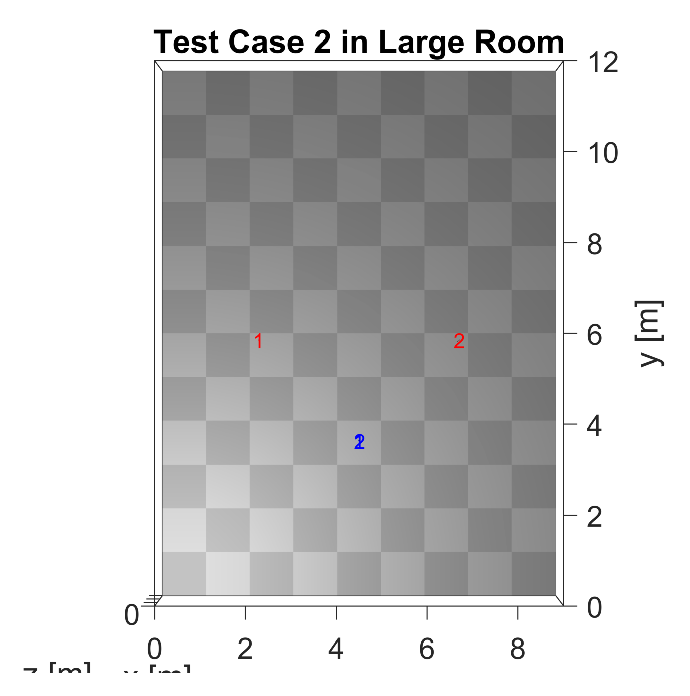
\includegraphics[width=\textwidth]{2l_lo}
\caption{Test Case 2}
\end{subfigure}
\begin{subfigure}[H]{0.45\textwidth}
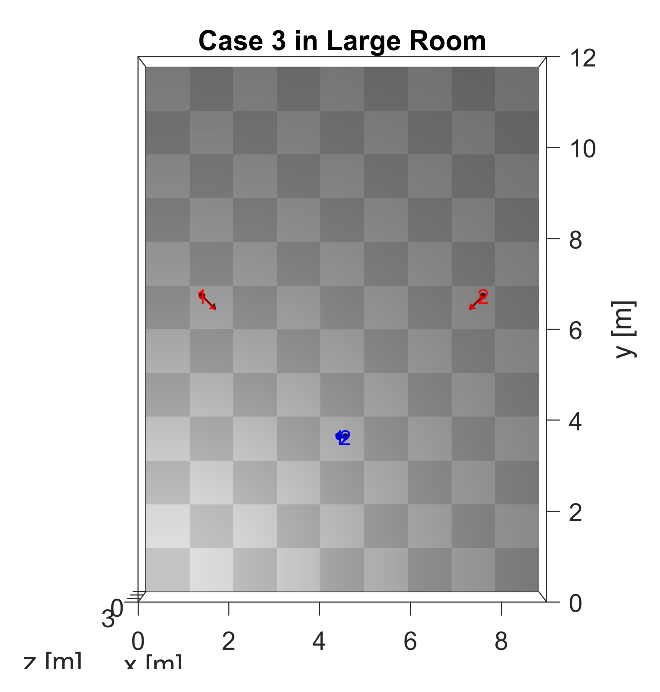
\includegraphics[width=\textwidth]{3l_lo}
\caption{Test Case 3}
\end{subfigure}
\caption{Source-Receiver Layout of Different Test Cases in a Large Room (Arrow represents the Direction of Speech)}
\label{fig:testcases}
\end{figure}

To investigate the effect of the reverberation on the audio zooming algorithm, three sizes of room are chosen - small, medium and large, as seen from Table \ref{table:roomsize}. The choice of room dimensions are designed with reference to \cite{AstolfiGoodPrivacy}, which aims to replicate situations such as taking videos in restaurants or in a conference. This forms the 9 test cases in total, which serves as the benchmark to evaluate the algorithm. (Refer to Appendix \ref{appendixresult} for all 9 test cases and the corresponding Room Impulse Response)

\begin{table}[H]
\centering
\begin{tabular}{|l|c|c|c|}
\hline
Room Dimension (m) & Width & Length & Height \\ \hline
Small & 3 & 4 & 3 \\ \hline
Medium & 6 & 8 & 3 \\ \hline
Large & 9 & 12 & 3 \\ \hline
\end{tabular}
\caption{Room Sizes adopted in the Testbench}
\label{table:roomsize}
\end{table}

The reverberation time \texttt{T30} is also plotted in Figure \ref{fig:reverb} to verify the results, which indicates that reverberation time increases for a larger room as expected. Comparing with reverberation time \texttt{T30} of a typical office room, which is around 150-200ms, the results are deemed reasonable and successful.

\begin{figure}[H]
\centering	
\begin{subfigure}[H]{0.3\textwidth}
\includegraphics[width=\textwidth]{t30s}
\caption{Small Room}
\end{subfigure}
\begin{subfigure}[H]{0.3\textwidth}
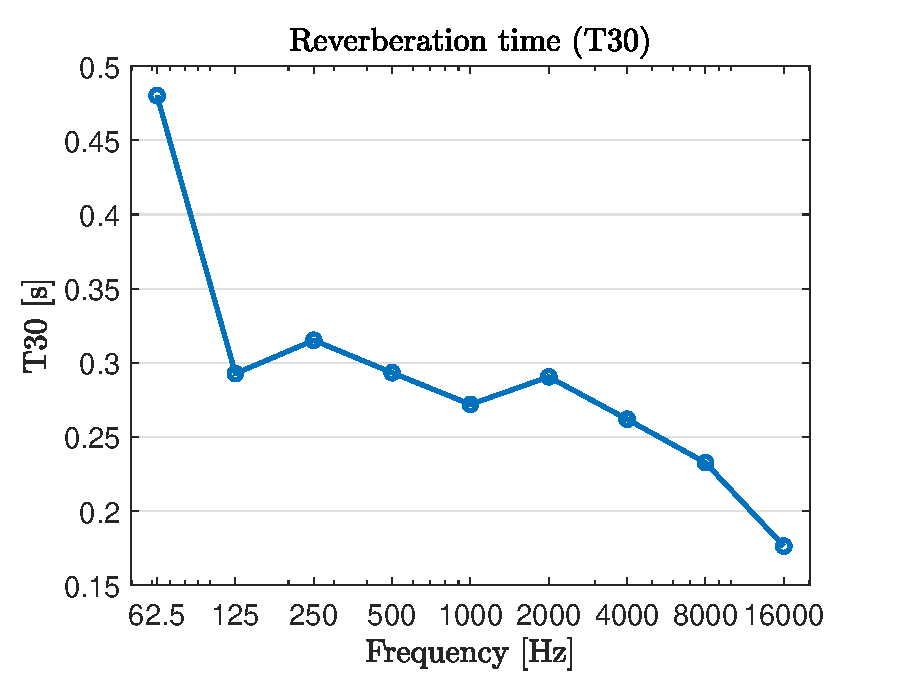
\includegraphics[width=\textwidth]{t30m}
\caption{Medium Room}
\end{subfigure}
\begin{subfigure}[H]{0.3\textwidth}
\includegraphics[width=\textwidth]{t30l}
\caption{Large Room}
\end{subfigure}
\caption{Reverberation Time \texttt{T30} in different room sizes}
\label{fig:reverb}
\end{figure}

\subsubsection{Outcome}
After developing the software and designing the test cases (Refer to Appendix \ref{appendixcode} for code listing), the last step is to generate the Room Impulse Response and use it to filter the audio data. Figure \ref{fig:outcome} shows the result from one of the test cases. From the Source-receiver layout, it can easily be seen that the room impulse response of source 1 at receiver 1 should be similar to the one of source 2 at receiver due to symmetry, which is verified through the plot. 
\begin{figure}[H]
\centering
\begin{subfigure}[H]{0.44\textwidth}
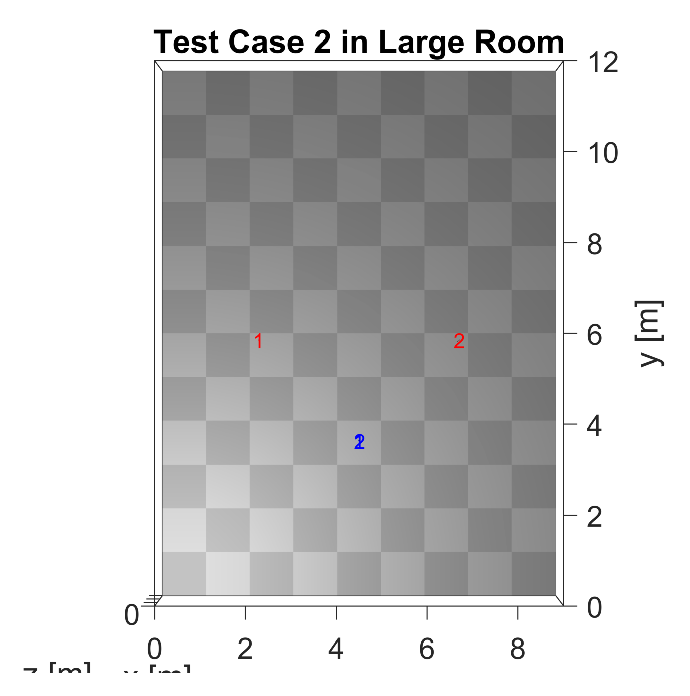
\includegraphics[width=\textwidth]{2l_lo}
\end{subfigure}
\begin{subfigure}[H]{0.55\textwidth}
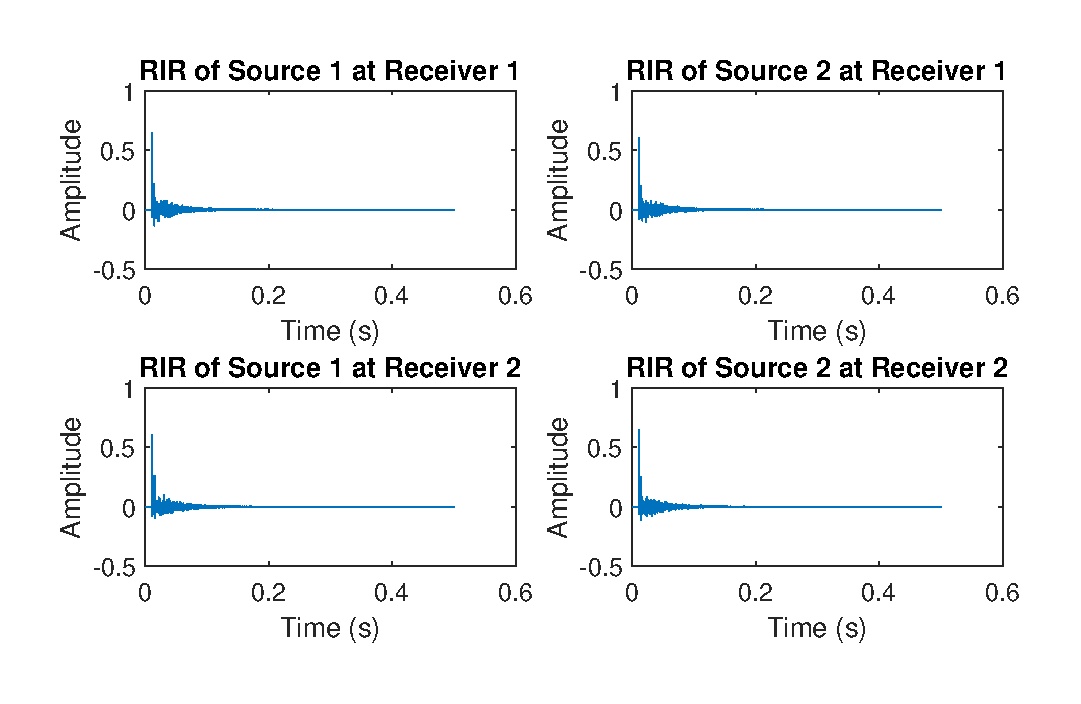
\includegraphics[width=\textwidth]{2l_ir}
\end{subfigure}
\caption{Source-Receiver Layout and Room Impulse Response of Test Case 2 in a Large Room}
\label{fig:outcome}
\end{figure}

Upon filtering the room impulse response with the anechoic speech, the spectrogram is then compared in Figure \ref{fig:spectreceived} \footnote{Spectrogram is generated using Hamming window of $N_w = 512$, with an overlapping factor of 2 under sampling frequency of 16kHz}. It can be seen that the received spectrogram is a mixture/combination of both anechoic speech as expected. Another observation is that the spectrogram of the received mixture appears to be more `blurry'. It is hypothesised that the phenomenon is due to the reverberation of the room, or in other words, the `echo' produced from one's speech.

\begin{figure}[H]
\centering	
\begin{subfigure}[H]{0.48\textwidth}
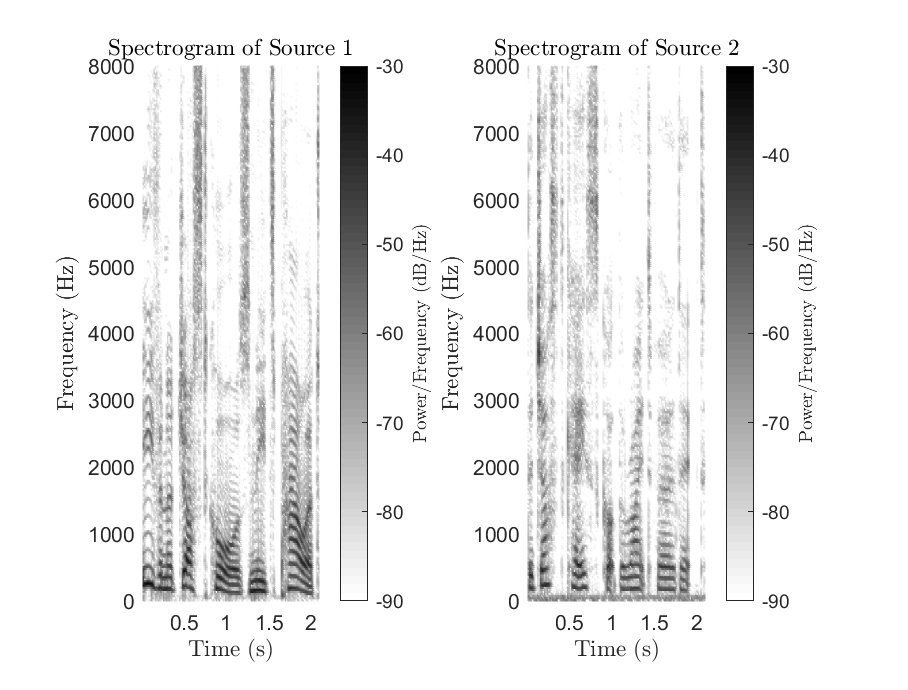
\includegraphics[width=\textwidth]{spectsrc}
\caption{Original Anechoic Speech}
\end{subfigure}
\begin{subfigure}[H]{0.48\textwidth}
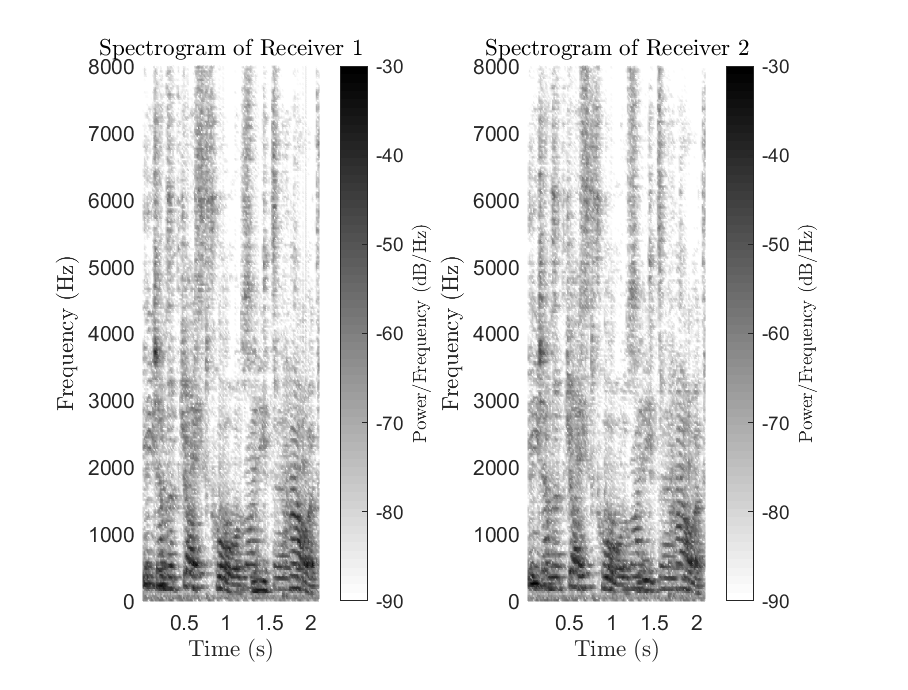
\includegraphics[width=\textwidth]{spectrec}
\caption{Received Mixture of Speech Signals}
\end{subfigure}
\caption{Comparison of Spectrogram of the Original Sound Source with the Received Sound in Test Case 2 in a Large Room}
\label{fig:spectreceived}
\end{figure}

\subsection{Phase II - Developing Processing Algorithm}
\subsubsection{Experimenting with Binary Masking}
With the simulated audio data available, the next step is moving onto the processing stage to develop the algorithm using time-frequency mask based on the phase difference. In this section, the context of the discussion focuses on Test Case 2 in a Large Room, as it is still under development stage.

The software has been developed under the help of \texttt{VOICEBOX} \cite{Brookes1997VOICEBOX:MATLAB.}, particularly with the routines \texttt{enframe.m} and \texttt{overlapadd.m}, which split signal up into overlapping frames, and combine them back together using overlap-add method after processing respectively. In this time-frequency analysis, the simulated audio signal received by the two microphones is first split into time frames using Hamming window of $N_w = 512$, with an overlapping factor of 2 under sampling frequency of 16kHz. In other words, the signals has been split into overlapping time-frame of $t=\frac{512}{16000}=32$ms.

Moving onto the binary mask, the approach adopted currently is the ``naive'' binary mask. It is obvious that from test case 2 that Source 1 will arrive at receiver 1 before receiver 2, and vice versa for Source 2. Therefore, by finding the time difference of arrival comparing the signals received by both microphones, each time-frequency bin can be labelled as from Source 1 or Source 2, which then forms the binary mask. As mentioned in the narrowband assumption, time difference of arrival is equivalent to the phase difference of arrival. A negative phase difference corresponds to a delay, while positive phase difference is equivalent to a lead. Hence, using receiver 1 as the reference receiver, by finding the phase difference of the time-frequency bins between two receivers, the time-frequency bins can be labelled, where ones with negative phase difference are labelled Source 1 and vice versa.

For example, the ``naive'' binary mask to zoom in Source 2 in Test Case 2 is formally defined as follows: 
\[
M_j(\tau,\omega) = \begin{cases} 1, & \text{if } \theta_j>0 \\ 0, & \text{otherwise} \end{cases}
\]
, where $\theta_j$ refers to the phase difference of the $j$-th time-frequency bin of receiver 2 with respect to receiver 1. Applying the binary time-frequency mask, the results are shown below.

\begin{figure}[H]
\centering	
\begin{subfigure}[H]{0.45\textwidth}
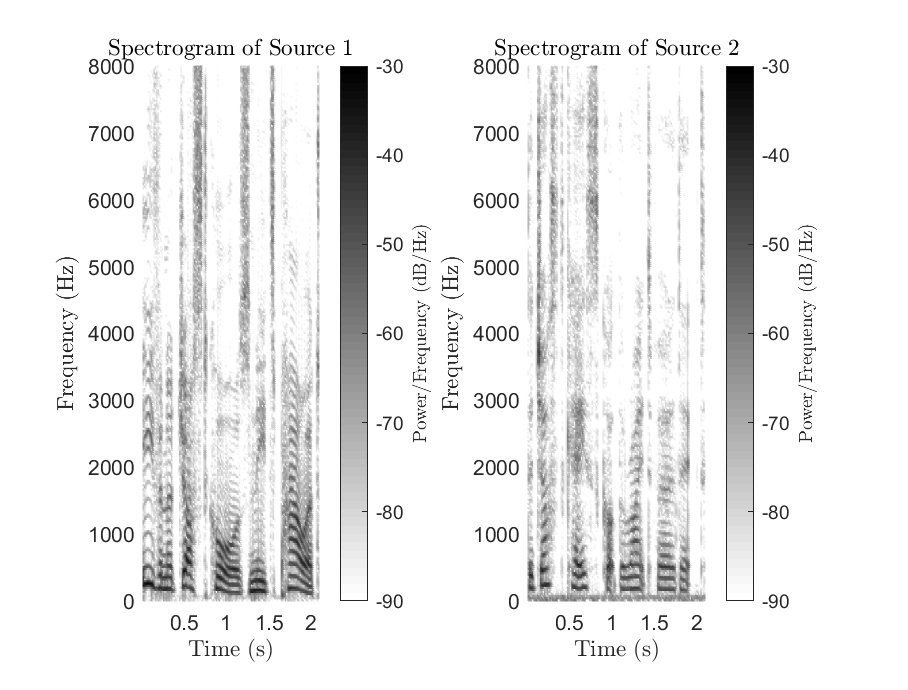
\includegraphics[width=\textwidth]{spectsrc}
\caption{Original Anechoic Speech}
\end{subfigure}
\begin{subfigure}[H]{0.45\textwidth}
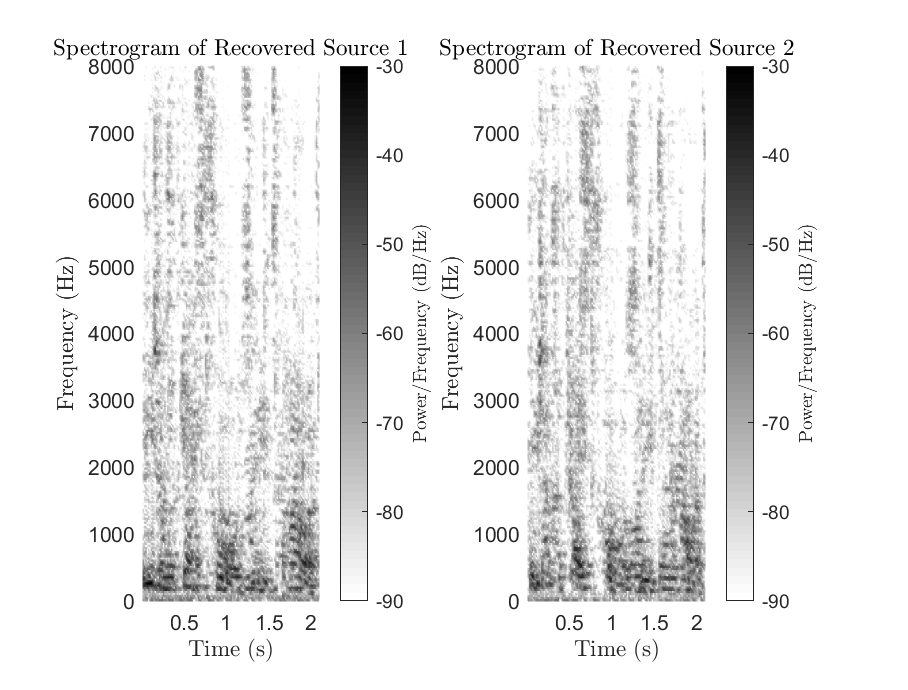
\includegraphics[width=\textwidth]{spectproc}
\caption{Masked Reverberant Speech}
\label{fig:masked}
\end{subfigure}
\caption{Comparison of Spectrogram of the Original Sound Source with the Processed Sound Source in Test Case 2 in a Large Room}
\label{fig:speccomp}
\end{figure}

From the Time-Frequency Analysis, by comparing the original Anechoic Speech and the masked received speech, it can be seen the binary masking has huge room for improvement. Despite some satisfactory results, such as the dark region at around $t=1$ for Source 1, the binary masks actually introduce distortion to the speech signal, as seen from the discontinuous dark spots in Figure \ref{fig:masked}. The reason behind is a the strong correlation between neighbouring time-frequency bins. As studied by \cite{Faller2004SourceCoherence}, the dominant parts of speech signals also form patches and are not randomly scattered across the time-frequency plane. It shows the need of clustering techniques, which will be discussed in Section \ref{futureworks}.

Another point of interest is the degree of suppression. Instead of a source separation problem, this project focuses on audio zoom, which does not necessarily mean that the interfering source should be completely removed, which may eventually sound unnatural to human ears. Hence, to improve from the ``naive'' binary mask, the degree of suppression of the interfering sources has to be revised.

\subsection{Summary}
In the beginning three months of the project, the main contribution has been on Phase I - Capturing Audio Data and Establishing Testbench. The results was deemed satisfactory with the reverberant audio data successfully generated. The work on Phase II - Developing Processing Algorithm has also started with background researches on some existing processing techniques like binary oracle masks and time-frequency analysis using spectrogram.
\newpage
\section{Future Works}
\label{futureworks}
Following the works on binary masks, in short-term, the focus would be to improve the criteria of binary masking by investigating the spectrogram for phase difference followed by clustering the time-frequency bins. The potential of incorporating other established techniques would also be explored.

In the long-term, following the project plan, the evaluation metrics would be decided. The performance would then be compared against some similar algorithms, and refinements would be made accordingly. As the final deliverable, a successful demonstration of the algorithm on simulated data (and real-life data captured by smartphones containing multiple speakers as a step forward) is expected. 

\subsection{Strategy}
To achieve the aforementioned goals, in the remainder of the project, various strategies would be taken place. First, same as the current approach, a strong communication link between project supervisor and myself should be maintained, in order to make sure the whole project is progressing in the right direction and pace as expected. This is achieved through bi-weekly and ad-hoc individual meetings with the project supervisor. Not only would close communications help myself understand the next steps of the project, it also allows project supervisor to monitor the overall progress of the project and make corresponding decisions. 

In addition, it is also a useful strategy to document every research results and idea development. Throughout this project, logbook has been used to write down daily and weekly progress. Comparing with the timeline outlined by Gantt chart allows myself to have a clear view on my own progress, advocating the overall project management. 

\section{Conclusion}
In the first three months of the Final Year Project, progress have been made on capturing audio data, as well as developing a novel processing algorithm to perform audio zooming on mobile phones. A project plan has also been set up, with the ultimate target to demonstrate the use of the algorithm on real-life or even real-time data. For the remainder of the project, a detailed timeline with contingency plans has been laid out to make strides towards a successful project.

\newpage
\bibliography{Mendeley} 
\bibliographystyle{ieeetr}
\newpage
\listoffigures
\listoftables
\newpage
\begin{appendices}
\begin{landscape}
\section*{Appendix}
\appendix
\section{Detailed Gantt Chart}
\pagenumbering{arabic}% resets `page` counter to 1
\renewcommand*{\thepage}{A-\arabic{page}}
\begin{figure}[H]
\begin{center}
\includegraphics[width=\linewidth,frame]{gantt}
\end{center}
\caption{Detailed Gantt Chart}
\end{figure}
\clearpage
\end{landscape}

\pagenumbering{arabic}% resets `page` counter to 1
\renewcommand*{\thepage}{B-\arabic{page}}
\section{Code Listing}
\label{appendixcode}
\lstinputlisting[language=MATLAB,breaklines=true,caption=Main Script for Phase I,captionpos=b]{fyp.m}
\newpage
\pagenumbering{arabic}% resets `page` counter to 1
\renewcommand*{\thepage}{C-\arabic{page}}
\section{Results of Phase I from Test Cases}
\label{appendixresult}
This section displays the results from 9 test cases simulated in different room geometries and different source-receiver locations. \footnote{Speakers are labelled in red, while Microphones are labelled in blue.}
\begin{figure}[H]
\centering	
\begin{subfigure}[H]{0.4\textwidth}
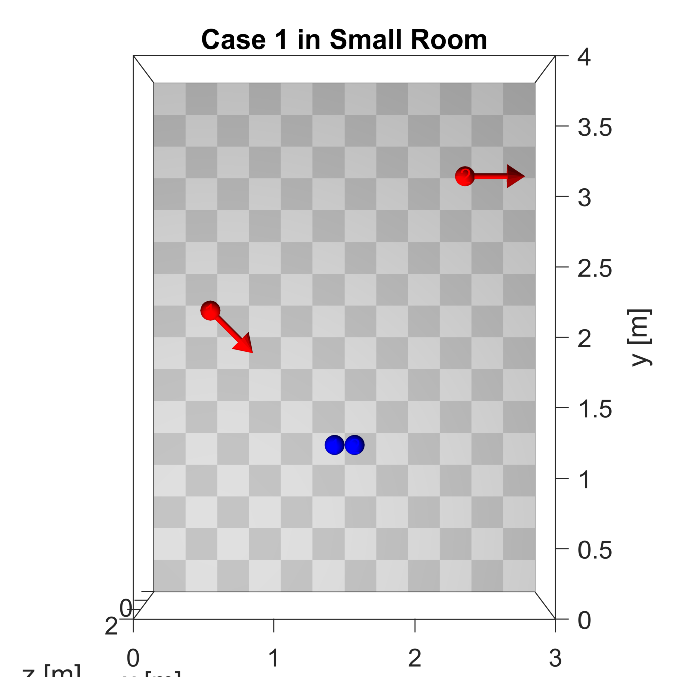
\includegraphics[width=\textwidth]{1s_lo}
\end{subfigure}
\begin{subfigure}[H]{0.45\textwidth}
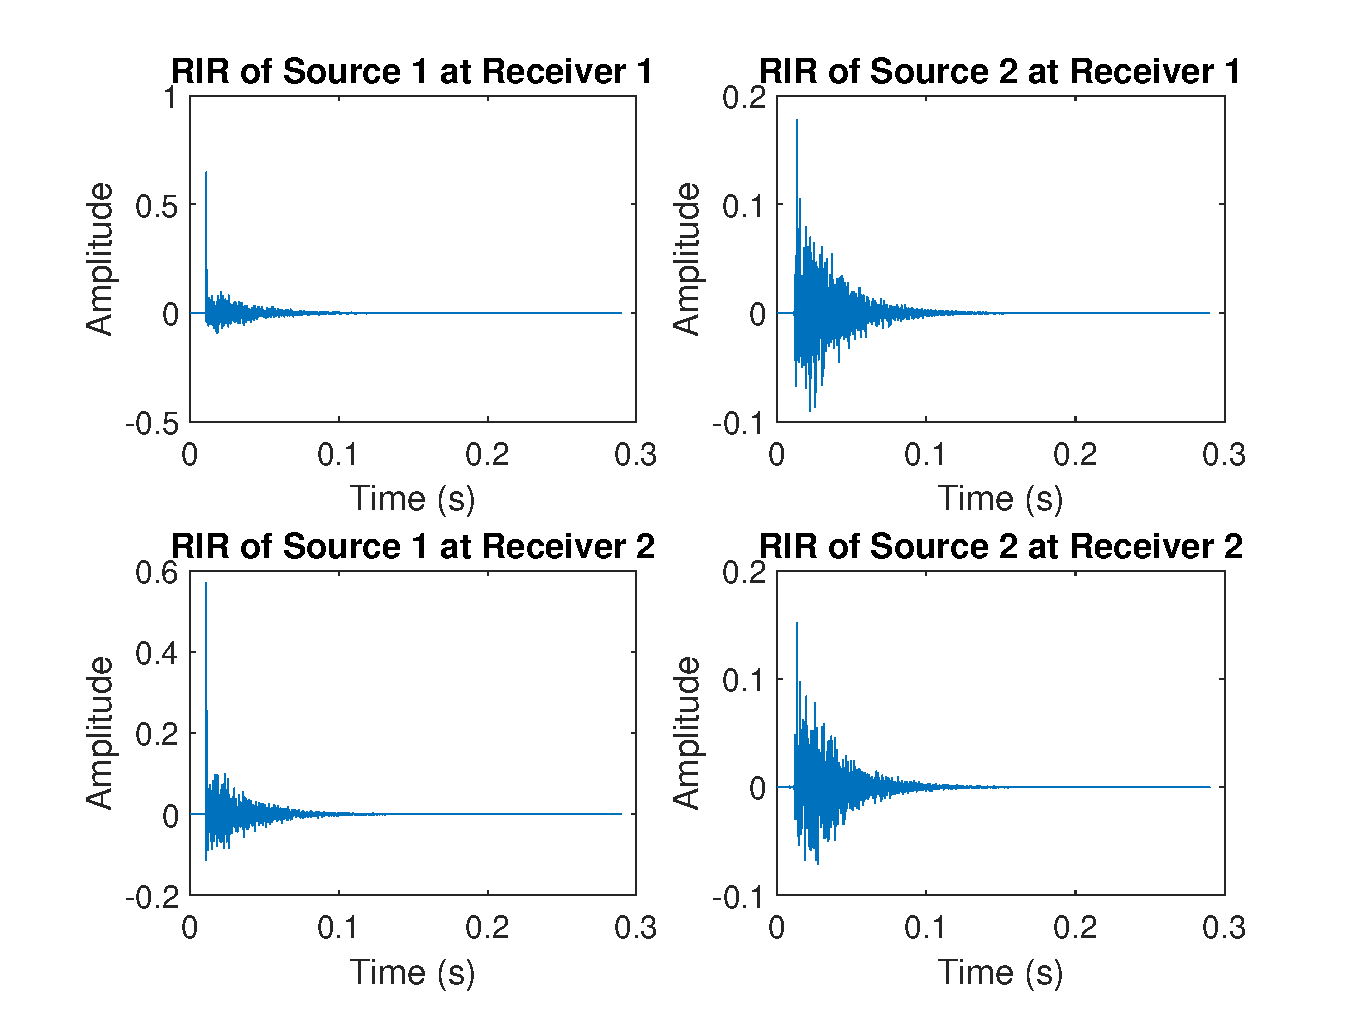
\includegraphics[width=\textwidth]{1s_ir}
\end{subfigure}
\caption{Room Layout and Room Impulse Response of Test Case 1 in a Small Room}
\end{figure}
\begin{figure}[H]
\centering
\begin{subfigure}[H]{0.4\textwidth}
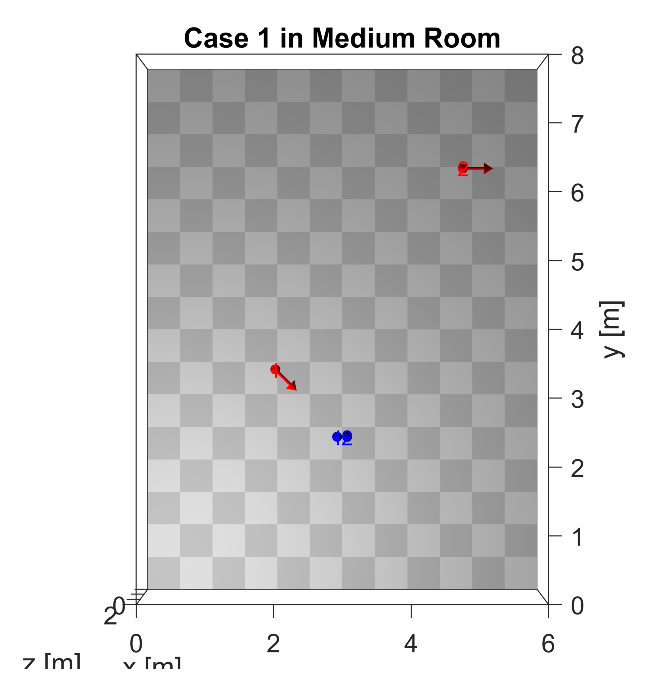
\includegraphics[width=\textwidth]{1m_lo}
\end{subfigure}
\begin{subfigure}[H]{0.45\textwidth}
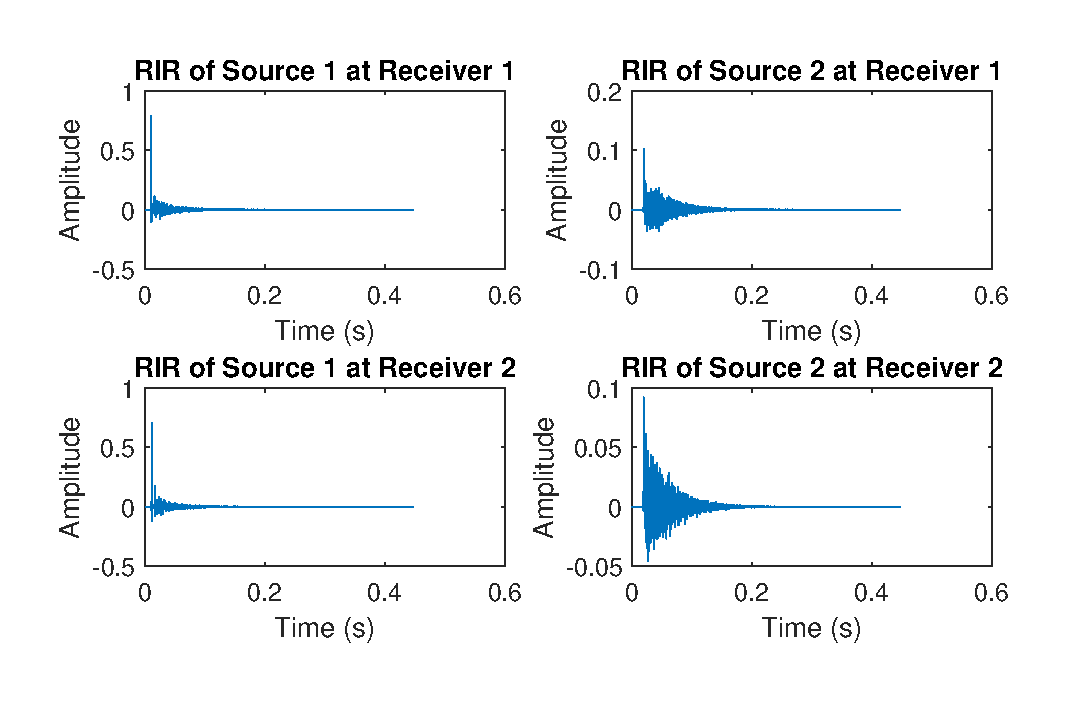
\includegraphics[width=\textwidth]{1m_ir}
\end{subfigure}
\caption{Room Layout and Room Impulse Response of Test Case 1 in a Medium Room}
\end{figure}
\begin{figure}[H]
\centering
\begin{subfigure}[H]{0.4\textwidth}
\includegraphics[width=\textwidth]{1l_lo}
\end{subfigure}
\begin{subfigure}[H]{0.45\textwidth}
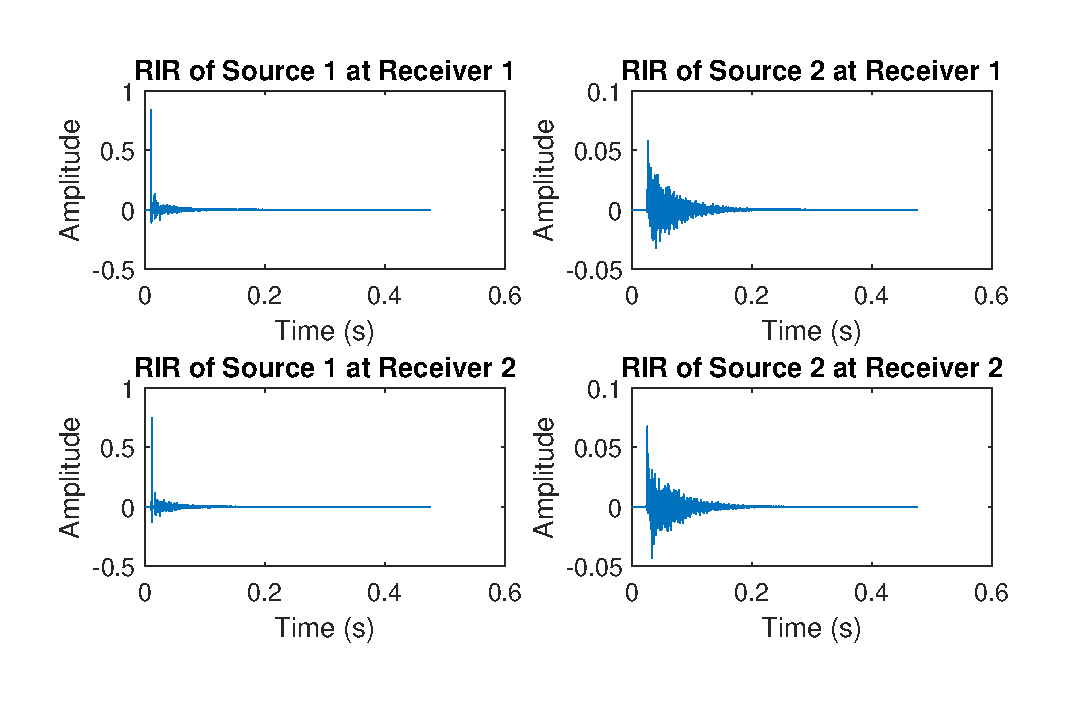
\includegraphics[width=\textwidth]{1l_ir}
\end{subfigure}
\caption{Room Layout and Room Impulse Response of Test Case 1 in a Large Room}
\end{figure}
\newpage
\begin{figure}[H]
\centering
\begin{subfigure}[H]{0.44\textwidth}
\includegraphics[width=\textwidth]{2s_lo}
\end{subfigure}
\begin{subfigure}[H]{0.55\textwidth}
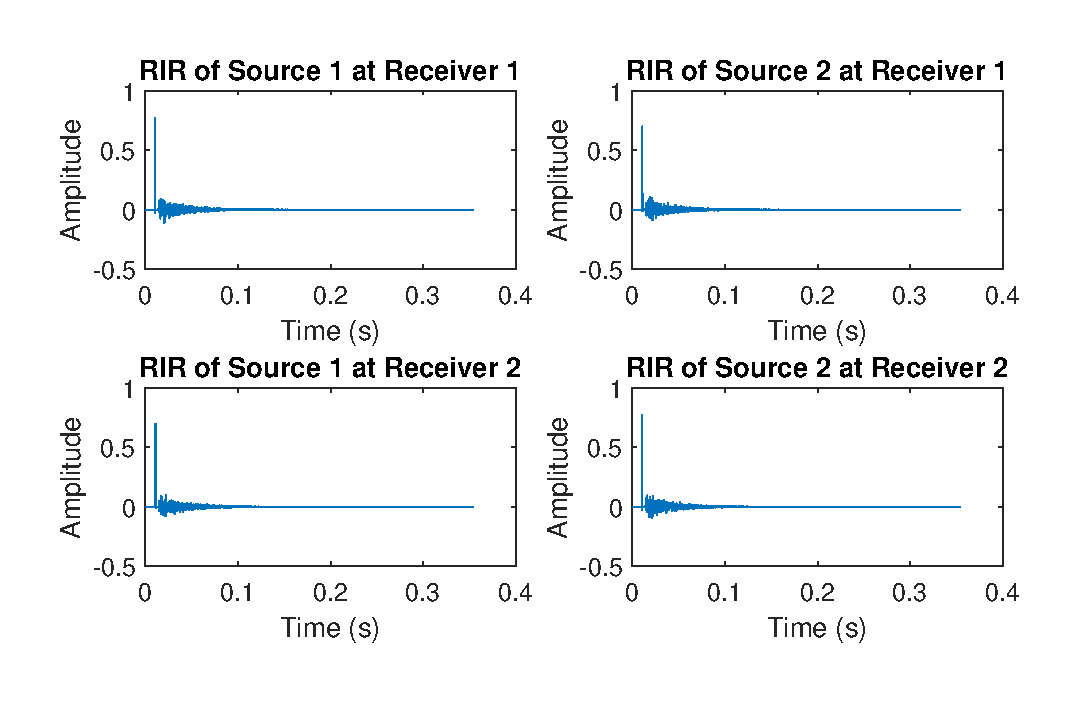
\includegraphics[width=\textwidth]{2s_ir}
\end{subfigure}
\caption{Room Layout and Room Impulse Response of Test Case 2 in a Small Room}
\end{figure}
\begin{figure}[H]
\centering
\begin{subfigure}[H]{0.44\textwidth}
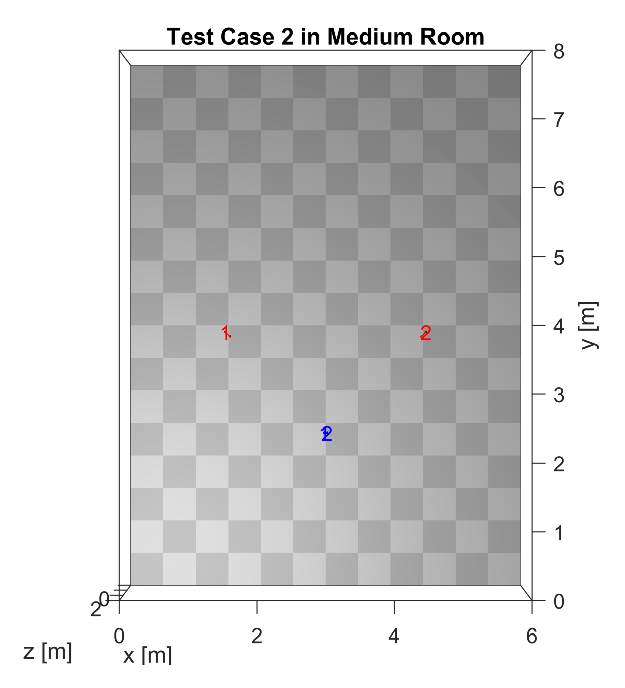
\includegraphics[width=\textwidth]{2m_lo}
\end{subfigure}
\begin{subfigure}[H]{0.55\textwidth}
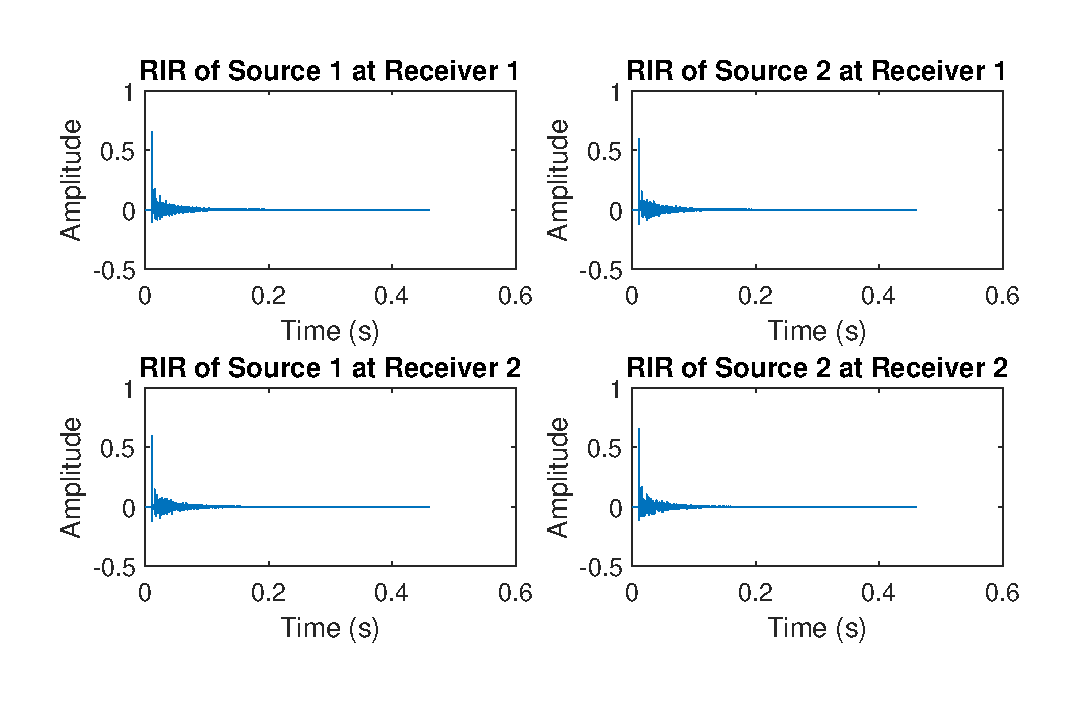
\includegraphics[width=\textwidth]{2m_ir}
\end{subfigure}
\caption{Room Layout and Room Impulse Response of Test Case 2 in a Medium Room}
\end{figure}
\begin{figure}[H]
\centering
\begin{subfigure}[H]{0.44\textwidth}
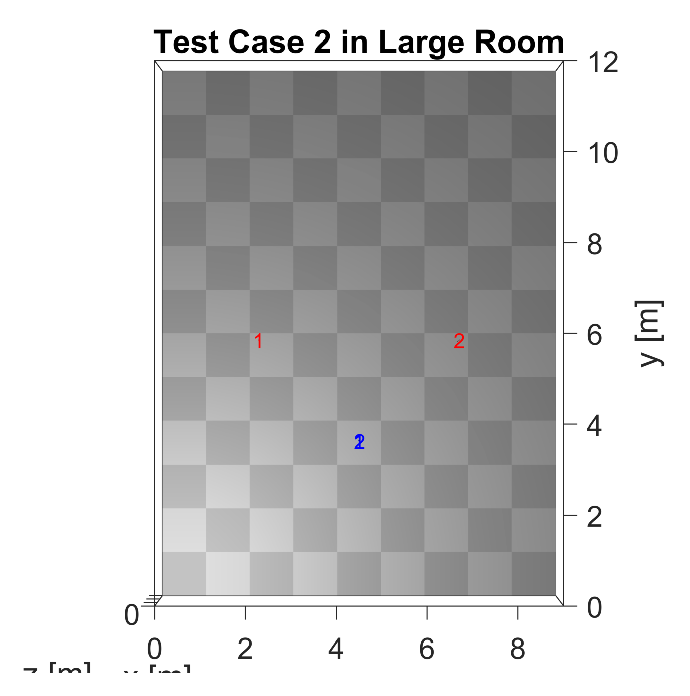
\includegraphics[width=\textwidth]{2l_lo}
\end{subfigure}
\begin{subfigure}[H]{0.55\textwidth}
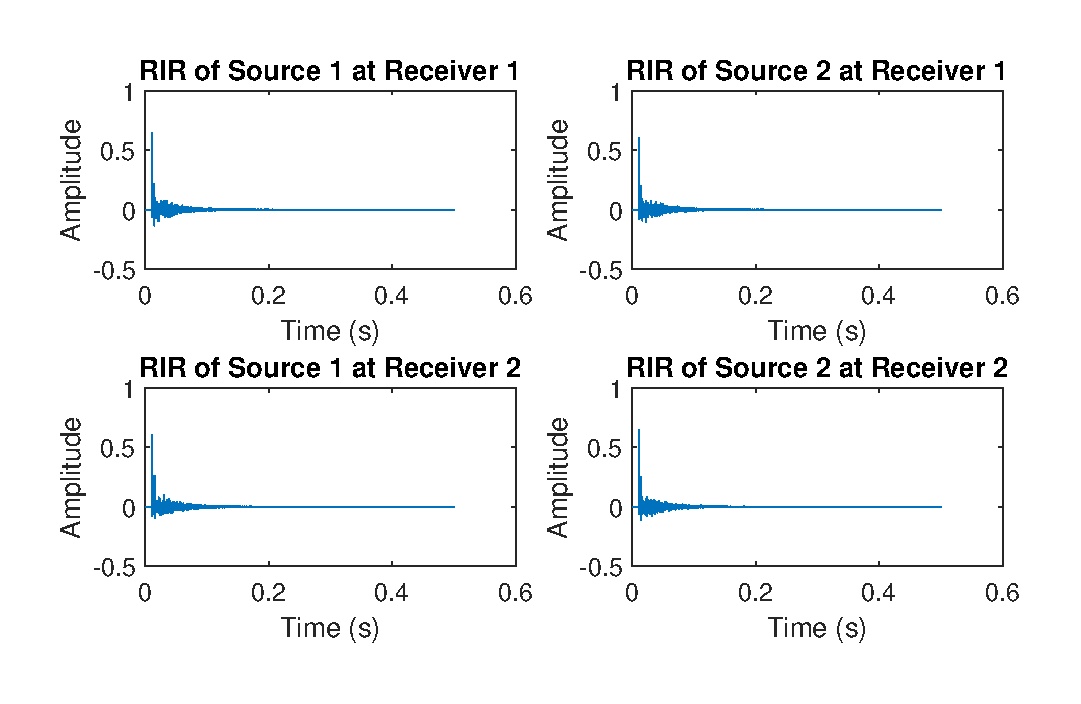
\includegraphics[width=\textwidth]{2l_ir}
\end{subfigure}
\caption{Room Layout and Room Impulse Response of Test Case 2 in a Large Room}
\end{figure}
\newpage
\begin{figure}[H]
\centering
\begin{subfigure}[H]{0.44\textwidth}
\includegraphics[width=\textwidth]{3s_lo}
\end{subfigure}
\begin{subfigure}[H]{0.55\textwidth}
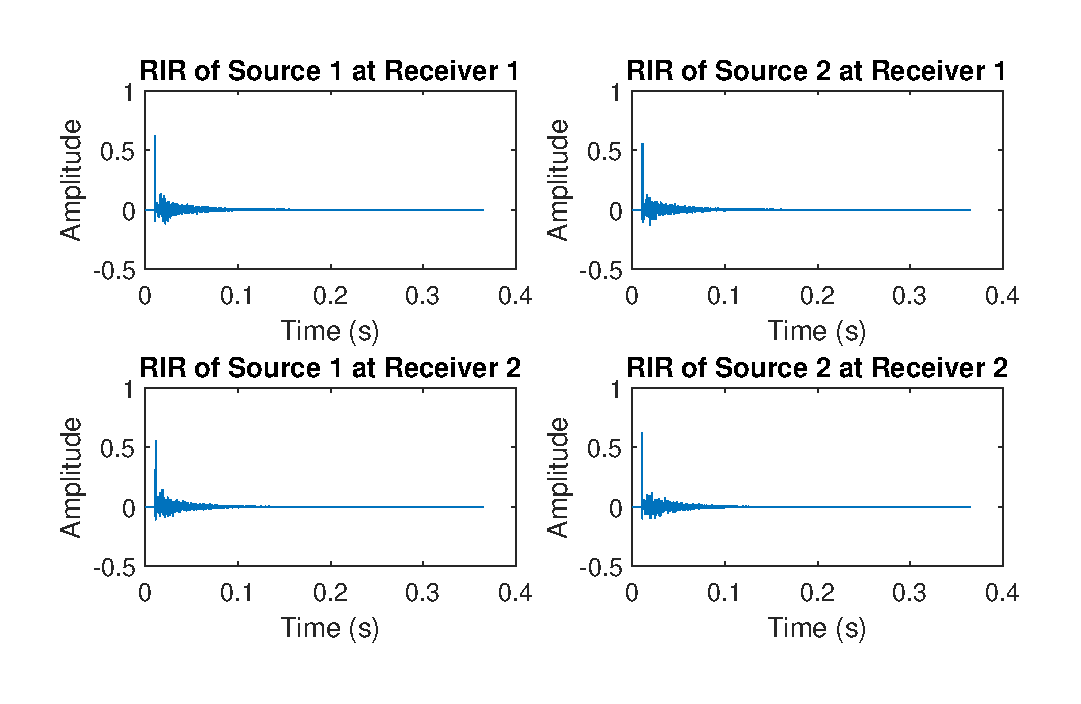
\includegraphics[width=\textwidth]{3s_ir}
\end{subfigure}
\caption{Room Layout and Room Impulse Response of Test Case 3 in a Small Room}
\end{figure}
\begin{figure}[H]
\centering
\begin{subfigure}[H]{0.44\textwidth}
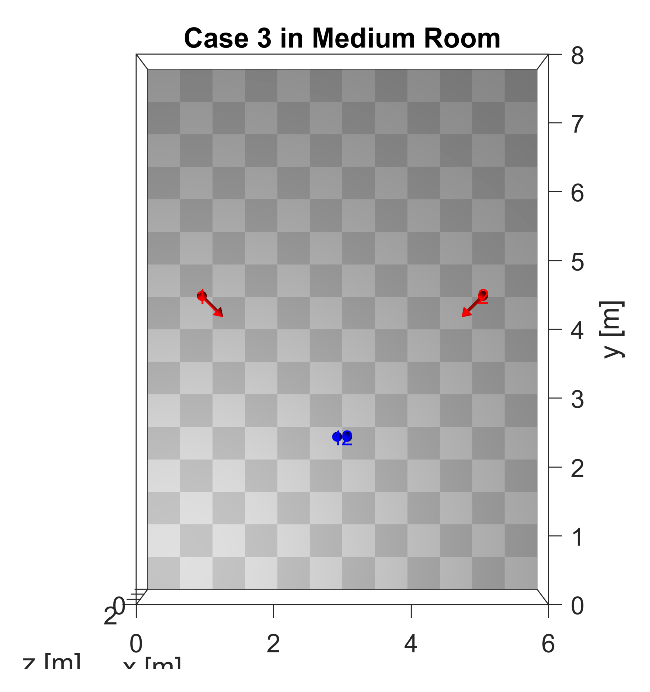
\includegraphics[width=\textwidth]{3m_lo}
\end{subfigure}
\begin{subfigure}[H]{0.55\textwidth}
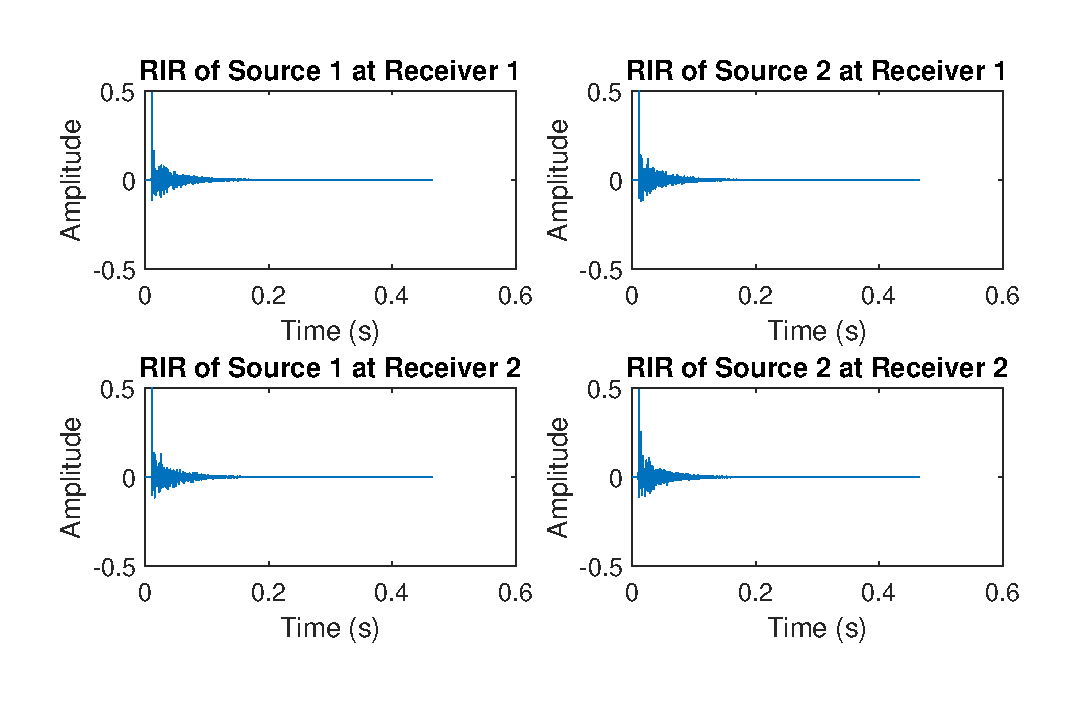
\includegraphics[width=\textwidth]{3m_ir}
\end{subfigure}
\caption{Room Layout and Room Impulse Response of Test Case 3 in a Medium Room}
\end{figure}
\begin{figure}[H]
\centering
\begin{subfigure}[H]{0.44\textwidth}
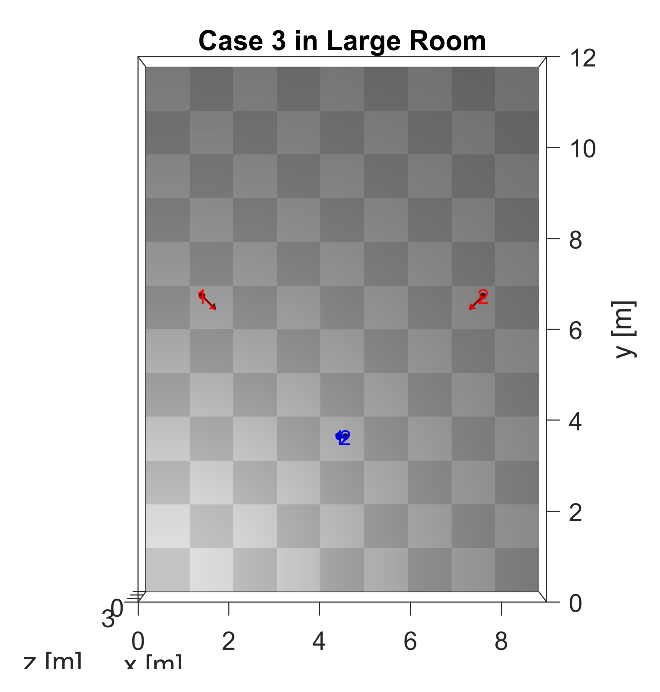
\includegraphics[width=\textwidth]{3l_lo}
\end{subfigure}
\begin{subfigure}[H]{0.55\textwidth}
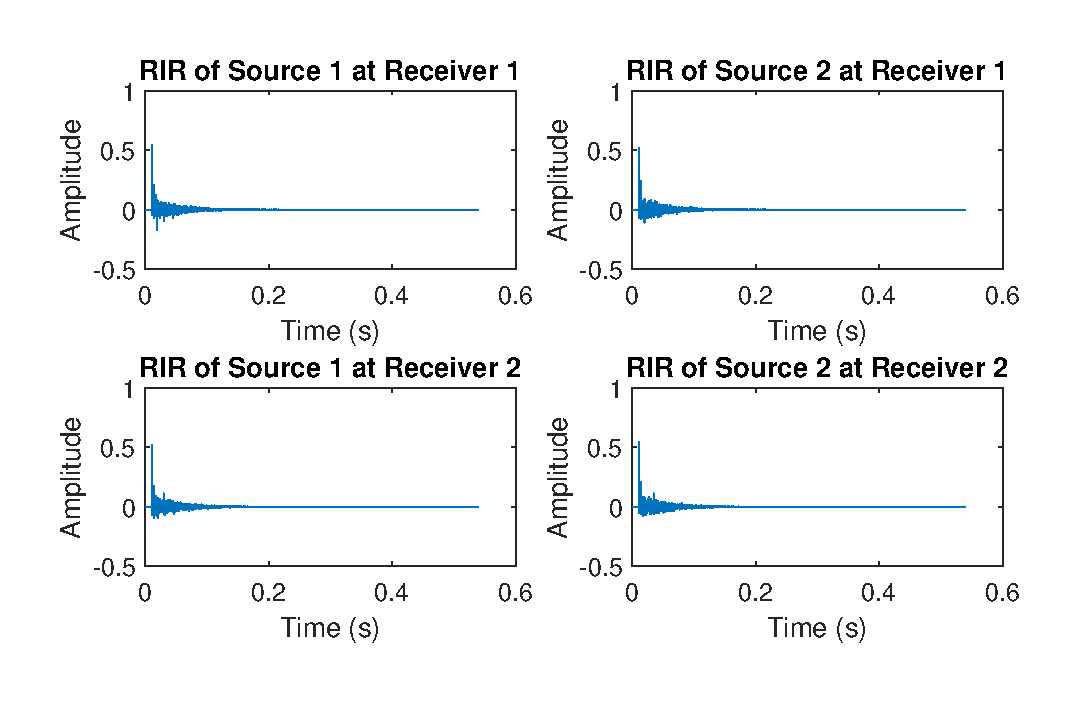
\includegraphics[width=\textwidth]{3l_ir}
\end{subfigure}
\caption{Room Layout and Room Impulse Response of Test Case 3 in a Large Room}
\end{figure}
\clearpage
\end{appendices}
\end{document}
